\section{Survey of approximate matching techniques}
Approximate matching is in general more complicated than exact matching. We can consider exact matching problems as a subset of approximate matching problems with an error of 0. The problem set will also change a lot if we use a different definition of the error metric or the type of errors. The time complexity of many efficient exact matching algorithms that work as simulating a DFA, such as the Knuth–Morris–Pratt algorithm, will become exponential as the number of errors grows if we just convert the NFA of the pattern into a DFA to be adapted in these algorithms. 

\begin{comment}

\subsection{Dynamic programming}

One of the classical solutions to approximate matching problem is to use dynamic programming. This method is simple and easy to be implemented by programming. 

% TODO: some examples maybe


\subsection{Autamata simulation}
Another classical one is automata simulation. The algortihm BNDM  (we will explain later) over which NR-grep is built is basically a simulation of an NFA. 

\end{comment}


\subsection{NR-grep}

\subsubsection{Bit-parallelism}
From the experiment results shown in the previous section, we can say in general NR-grep has the best performance in average in our various test cases. This is not surprising because NR-grep implemented different efficient algorithms for various pattern matching problems as well as a good software design. From this tool's perspective, the patterns are classified into three levels: simple patterns, extended patterns and regular experssions. Different algorithms are applied to different levels of patterns to make sure that the problem can be solved in the most efficient way. 

We now show the idea of how NR-grep solves the approximate matching in an efficient way. The name of this tool comes from "nondeterministic reverse $grep$", which indicates this tool can simulate NFAs instead of converting them to DFAs. The algorithm of  simulating NFAs used in NR-grep is called $Shift-Or$. This algorithm is based on an approach called $bit-parallelism$, which takes advantage of the parallelism of the bit operations inside a computer word. A variant of Shift-Or that is easier to explain is $Shift-And$ algorithm, which also based on $bit-parallelism$. We first show how this algorithm works. 

Given a pattern $pat$ of length $m$,  and a text $txt$ of length $n$ and the alphabet set is $\Sigma$ with a size $|\Sigma|$. First we build a table $B$ in which for each character in $\Sigma$ stores a bit mask $b_m...b_1$. Each bit mask in the table has a length of $m$. For a character $char$ in $pat$ with an index $i$ (1-indexed), set the $m-i-1$ bit of the mask in B[$char$]. The following example shows a bit mask table for the pattern "abc" assuming $\Sigma$ = {a,b,c,d}.


\begin{example}\emph{The bit mask table for pattern "abc".}

\begin{table}[H]
	\centering
	\begin{tabular}{|c|c|c|c|}
		\hline
		index      & 1                        & 2                        & 3                        \\ \hline
		\textbf{a} & 0                        & 0                        & {\color[HTML]{3531FF} 1} \\ \hline
		\textbf{b} & 0                        & {\color[HTML]{3531FF} 1} & 0                        \\ \hline
		\textbf{c} & {\color[HTML]{3531FF} 1} & 0                        & 0                        \\ \hline
		\textbf{d} & 0                        & 0                        & 0                        \\ \hline
	\end{tabular}
	\label{table-bitmask}
\end{table}
\end{example}

We use a computer word $D = d_m...d_1$ to store the current active state with an initial value of all bits 0. During the searching process, $D$ is updated with the following formula: 
$$D' \leftarrow ((D << 1) \ | \ 0^{m-1}1) \ \& \ B[t_j]$$
where $t_j$ is the next text character.  When the $d_m$ bit in $D$ is set, we report the match. 

One of the advantages of the $Shift-Or$ algorithm is that it is easy to be extended to handle classes of characters, which is helpful for approximate matching. 
For example, we can now search for the pattern "ab."\footnote{ We use symbol '.' in this report to stand for a wildcard.}, which can be considered as the pattern "abc" allows a replacement error at the third character by just setting the $m-3+1$ bit of all the characters in the bit mask table as the following example shows. 

\begin{example}\emph{The bit mask table for pattern "ab."}.
	\begin{table}[H]
		\centering
		\begin{tabular}{|c|c|c|c|}
			\hline
			index      & 1                        & 2                        & 3                        \\ \hline
			\textbf{a} & {\color{red} 1}                   & 0                        & {\color[HTML]{3531FF} 1} \\ \hline
			\textbf{b} &  {\color{red} 1}                    & {\color[HTML]{3531FF} 1} & 0                        \\ \hline
			\textbf{c} & {\color[HTML]{3531FF} 1} & 0                        & 0                        \\ \hline
			\textbf{d} &{\color{red} 1}                    & 0                        & 0                        \\ \hline
		\end{tabular}
		\label{table-bitmask2}
	\end{table}
\end{example}

With this new bit mask table, searching for the pattern "ab.", or more generally a pattern that contains wildcards, will be just the same time complexity as search for "abc". 
%We can also find that an error of insertion can be dealt with by adding a new row of all 1s in the bit mask table and a deletion is just removing one row. 
 
\subsubsection{BNDM algorithm}
As we know, many efficient pattern matching algorithms, such as the Knuth–Morris–Pratt and the Boyer-Moore algorithm, employ a trick of skipping characters. It is possible to combine the $bit-parallelism$ approach with the ability of skipping characters to achieve an even more efficient algorithm. This idea is implemented by the $BNDM$ algorithm, which is used in NR-grep. BNDM uses $Shift-Or$ instead of $Shift-And$, a variant of $Shift-And$ that uses the following state updating formula:  
$$ D' \leftarrow  (D \ \& \ B[t_j]) << 1 .$$ The algorithm that is adapted in BNDM for skipping charaters is from the Boyer-Moore or the BDM families\cite{crochemore1994text}.


\subsubsection{NFA simulation}
As we have shown above, bit-parallelism deals with single error efficiently.
Now we present how bit-parallelism can be used to simulate an NFA for approximate matching. 

Consider the pattern "ab" allowing one error, we can build an NFA to simulate it as the follow figure shows.

\begin{figure} [H]
\begin{center}
	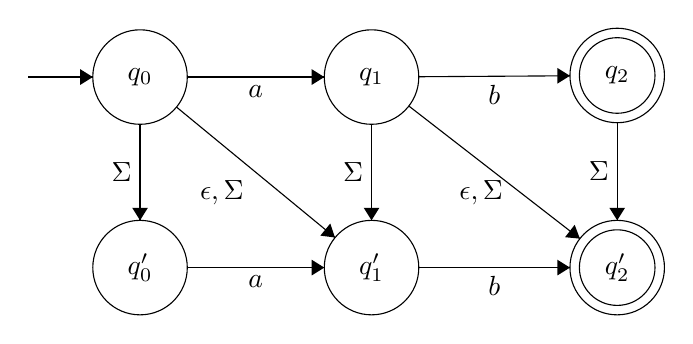
\begin{tikzpicture}[scale=0.2]
	\tikzstyle{every node}+=[inner sep=0pt]
	\draw [black] (18.3,-25.8) circle (3);
	\draw (18.3,-25.8) node {$q_0$};
	\draw [black] (33,-25.8) circle (3);
	\draw (33,-25.8) node {$q_1$};
	\draw [black] (18.3,-37.9) circle (3);
	\draw (18.3,-37.9) node {$q_0'$};
	\draw [black] (33,-37.9) circle (3);
	\draw (33,-37.9) node {$q_1'$};
	\draw [black] (48.6,-25.7) circle (3);
	\draw (48.6,-25.7) node {$q_2$};
	\draw [black] (48.6,-25.7) circle (2.4);
	\draw [black] (48.6,-37.9) circle (3);
	\draw (48.6,-37.9) node {$q_2'$};
	\draw [black] (48.6,-37.9) circle (2.4);
	\draw [black] (11.2,-25.8) -- (15.3,-25.8);
	\fill [black] (15.3,-25.8) -- (14.5,-25.3) -- (14.5,-26.3);
	\draw [black] (21.3,-25.8) -- (30,-25.8);
	\fill [black] (30,-25.8) -- (29.2,-25.3) -- (29.2,-26.3);
	\draw (25.65,-26.3) node [below] {$a$};
	\draw [black] (21.3,-37.9) -- (30,-37.9);
	\fill [black] (30,-37.9) -- (29.2,-37.4) -- (29.2,-38.4);
	\draw (25.65,-38.4) node [below] {$a$};
	\draw [black] (18.3,-28.8) -- (18.3,-34.9);
	\fill [black] (18.3,-34.9) -- (18.8,-34.1) -- (17.8,-34.1);
	\draw (17.8,-31.85) node [left] {$\Sigma$};
	\draw [black] (33,-28.8) -- (33,-34.9);
	\fill [black] (33,-34.9) -- (33.5,-34.1) -- (32.5,-34.1);
	\draw (32.5,-31.85) node [left] {$\Sigma$};
	\draw [black] (36,-25.78) -- (45.6,-25.72);
	\fill [black] (45.6,-25.72) -- (44.8,-25.22) -- (44.8,-26.22);
	\draw (40.8,-26.26) node [below] {$b$};
	\draw [black] (36,-37.9) -- (45.6,-37.9);
	\fill [black] (45.6,-37.9) -- (44.8,-37.4) -- (44.8,-38.4);
	\draw (40.8,-38.4) node [below] {$b$};
	\draw [black] (20.62,-27.71) -- (30.68,-35.99);
	\fill [black] (30.68,-35.99) -- (30.38,-35.1) -- (29.75,-35.87);
	\draw (23.49,-32.34) node [below] {$\epsilon, \Sigma$};
	\draw [black] (48.6,-28.7) -- (48.6,-34.9);
	\fill [black] (48.6,-34.9) -- (49.1,-34.1) -- (48.1,-34.1);
	\draw (48.1,-31.8) node [left] {$\Sigma$};
	\draw [black] (35.37,-27.64) -- (46.23,-36.06);
	\fill [black] (46.23,-36.06) -- (45.9,-35.18) -- (45.29,-35.97);
	\draw (39.96,-32.35) node [below] {$ \epsilon,\Sigma$};
	\end{tikzpicture}
\end{center}
\caption{An NFA accepting the pattern "ab" with at most one error. The label $\epsilon,\Sigma$ on the diagnoal arrows means both $\epsilon$ and $\Sigma$ can be accepted.}
\label{fig:nfa"ab"}
\end{figure}
 
In Figure \ref{fig:nfa"ab"}, the last state of each row stands for a state that accepts $r$ errors where $r$ is the index of the row (0-indexed). That is, in our example, the state $q_2$ accepts "ab" with no error and $q_2'$  with exact one error. The vertical arrows represent an insertion, and the $\epsilon$ and $\Sigma$ on the diagonal arrows stand for a deletion and a replacement respectively. We can image that we could build an NFA for any other patterns with $k$ errors in such manner iteratively. It is worth noting that the number of states in the NAF built in such a way increases linearly with the number of errors.

The technique stores each row in a machine word, say $R_i$ for row $i$ %just as we have shown in $Shift-And$.???
The updating of these words are performed with the following formulars: 

\begin{align*}
R_0' \leftarrow & ((R_0 << 1) \ |\ 0^{m-1}) \ \& \ B[t_j] \\
for \ &i \in 1...k \ do:  \\
	& R_i' \leftarrow ((R_i << 1) \ \& \ B[t_j] ) \ |\ R_{i-1} \ | \ (R_{i-1} << 1 ) \ |\ (R_{i-1}' << 1)
\end{align*}

These formulars show us one case of how bit-parallelism simulate an NFA. $R_0'$ is updated just as we have shown in $Shift-And$. In the formular for updating $R_i'$, the first element (i.e., $((R_i << 1) \ \& \ B[t_j] ) $ ) is similar to $Shitf-And$ but removed the OR operation with $O^{m-1}$ because it can not be an initial state that has a self-loop. The second is the old value of its upper row, which corresponds to a vertial arrow. Similarly, the third stands for a replacement and the fourth a deletion. When we detect that $R_k \& 10^{m-1}$ is set, a match is reported.  

As we can see from the above updating formulas, each updating is just bitwise operation hence constant time. So this simulation should be linear time complexity with $k$.
 
\subsection{Python (\texttt{regex})}

\subsection{Scan For Matches}


\subsection{Approximate Kleenex}